
\subsection{Datasets collection}


We build our CG dataset by collecting network packets with Wireshark (\textit{v3.6.2}). %\joel{je comprends pas ce que "live" apporte comme information.}
In a first campaign conducted in 2022, we considered the four main CG platforms available in Europe at that time: Nvidia GeForce Now (GFN), PlayStation Now (PSN), Google Stadia (STD) and Microsoft Xbox Cloud Gaming (XC). In a second dataset built in 2023, we collected data on GFN, PSN and XC in addition to Moonlight and Steam Remote Play (STD was shut down by Google in January 2023 but we keep STD data for comparison). The captures result in \texttt{pcap} files, all made available for the sake of reproducilibity\footnote{ \url{https://cloud-gaming-traces.lhs.loria.fr/data.html}}, from which we extract features. 

Marchal et al. \cite{marchal2023analysis} showed that most CG platforms adapt their traffic to network conditions. 
%\textcolor{blue}{
Typically, during congestion, CG platforms reduce their bitrate by increasing packet inter-arrival times (IATs) and/or decreasing packet sizes. 

% Dû à l'adaptation des plateformes -> baisse débit
To take these traffic variations into account, we also captured CG traffic under network constraints.  We add a router between the gateway and the CG client to alter the network conditions thanks to \textit{iproute} \texttt{tc} commands, and \textit{Wondershaper} for bandwidth limitation  (Fig. \ref{fig:chap_4:dataset_perturb}).  The generated network perturbations are applied in turn: (i) 20ms of additional delays; (ii) 5 ms of additional jitter; (iii) 5\% of packet loss; (iv) 10Mbps of available bandwidth. The host running the CG client performs the network capture.

\begin{figure}[!t]
    \centering
    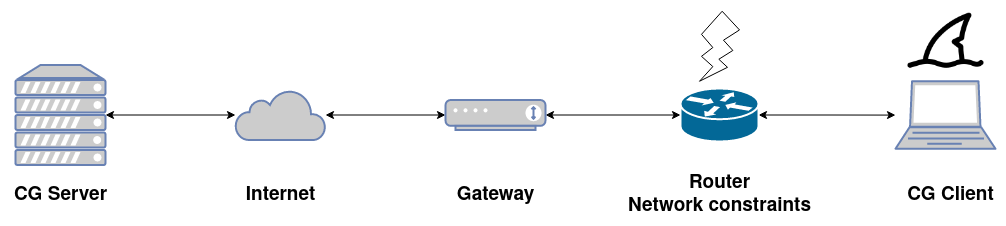
\includegraphics[scale=.4]{imgs/chapter_4/Perturb.png}
    \caption{Testbed for live network packets capture}
    \label{fig:chap_4:dataset_perturb}
\end{figure}

 
We also collect Non-Cloud Gaming (NCG) traffic by considering the following high-bandwidth traffic types over UDP; video streaming (VS), live video streaming (LV), video conferencing (VC), and Facebook navigation (FB) over QUIC. 
%Our datasets are available online\footnote{\url{cloud-gaming-traces.lhs.loria.fr}}. 
    % FEATURES 12 features
\par
We can then extract features from packet captures. 
Due to the asymmetry of CG traffic, we differentiate downlink and uplink features. 
For each direction, we extract six features per time window (we set its duration to 33 ms according to \cite{NOMS}): (1) the total number of packets, (2) the sum, (3) the mean and (4) the standard deviation of packet size, (5) the mean and (6) the standard deviation of packet inter-packet-arrival times (IAT).

% PLAN
% NCG
% Features 

\subsection{ML Models}
We formalize the CG traffic identification problem as a binary classification problem as follows. Given a dataset of traffic features $x_T = \{x_1, x_2, ..., x_n\}$, we train a model $\mathcal{M}$ which must assign for each new window of features observed $\tilde{x_i}$, a label among two classes within the set \{CG; NCG\}.% The problem can be formulated .

\subsubsection{DT Model limitations}

In our previous works \cite{NOMS}, we performed the identification of CG traffic using a \textit{Decision Tree} (DT) model which is a supervised machine learning approach. The goal of supervised learning is to learn the underlying mapping between a new observed instance $\tilde{x_i}$ and its respective label $\tilde{y_i}$, given a set of training examples $\{(x_1,y_1), ... (x_n,y_n)\}$, where $x_i$ and $y_i$ denote the feature vector and its label respectively. We trained the DT model using an equal proportion of CG and NCG instances. 
%\joel{Je me demande si je dois préciser ici le pourcentage de CG vs NCG instances avec éventuellement les différentes classes de service (streaming, live, visio...) utilisées dans l'entraînement}
The resulting DT model showed good performance for identifying CG traffic even when it was collected under downgraded network conditions. The DT model also classified efficiently NCG traffic types that were present in the training set. To assess the reliability of this model in an open world, we made a new dataset of unseen games executed on previously trained platforms as well as unseen CG platforms. Unfortunately, we realized that, when considering CG traffic not seen during training, the model performance declines (see Fig. \ref{fig:chap_4:usad_dt_comparison}, blue columns) to unacceptable proportions in the case of new platforms. %\joel{Référence des résultats du DT model sur des traces où il performe moins bien.}

\subsubsection{USAD Model}

To bypass the lack of generalization of our supervised model, we propose to identify CG traffic in an unsupervised manner. We use the USAD model (UnSupervised Anomaly Detection) \cite{audibert2020usad}, specifically designed for \textit{anomaly detection}, which employs a neural network architecture consisting of two auto-encoders: the model learns, based only on CG traffic features (without the label information), how to reconstruct the input data and compute a score $s$ measuring how efficient the model is in the reconstruction task. Since the model has learnt how to reconstruct only CG traffic features, it cannot perform an equivalent reconstruction of the NCG traffic. Hence, the NCG traffic will have a high reconstruction score while CG traffic will have a low reconstruction score. Then, given the reconstruction score $s$ computed by the model considering the features extracted from a given window $\tilde{x_i}$, and a carefully chosen threshold $\delta$, the window is classified as follows:

\begin{equation}
    \tilde{y_t} = 
    \begin{cases}
       CG, & \text{if } s(\tilde{x_t}) \leq \delta \\
       NCG, & \text{otherwise.}
    \end{cases}
\end{equation}

The rationale behind this strategy is to discriminate the CG traffic from the NCG traffic by relying not on a ground truth to learn discriminating rules  or relations but by using the latent characteristics of the dataset \cite{Johari2022AnomalyDA}. Therefore, the model should be more robust and more generalizable to unseen types of CG traffic. 

\begin{figure}[!t]
    \centering
    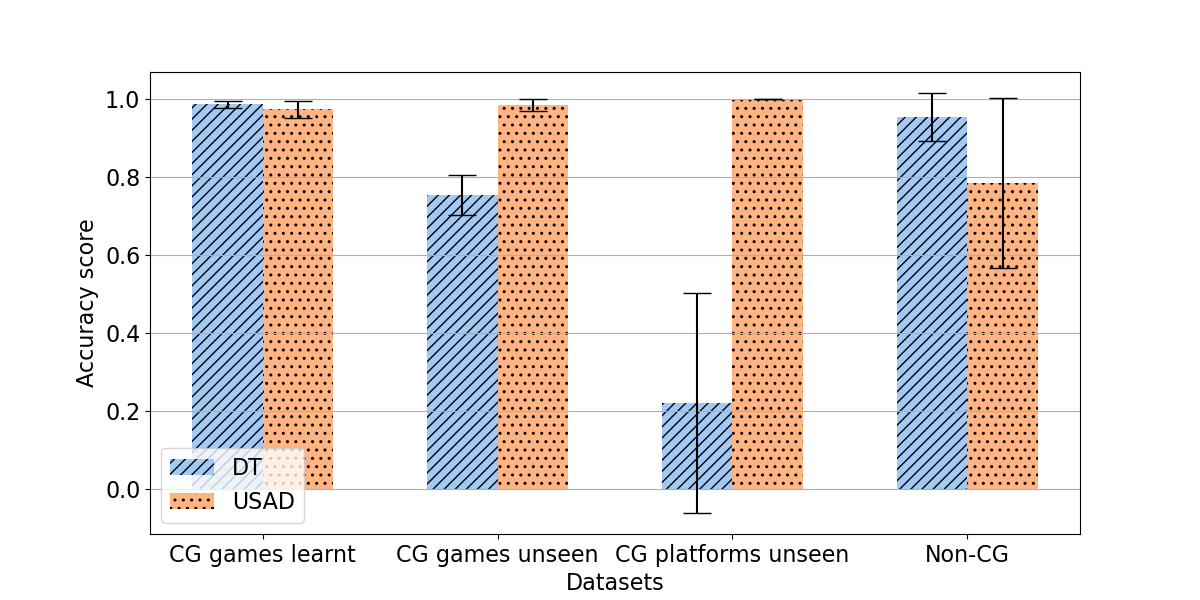
\includegraphics[width=.8\textwidth]{imgs/chapter_4/comparison_dt_usad.png}
    \caption{Performance of DT and USAD models}
    \label{fig:chap_4:usad_dt_comparison}
\end{figure}

%\subsection{USAD training procedure}
We split our CG dataset into a train and a test set as follows: the former is composed of normal CG instances from the 4 main CG platforms at our disposal (STD, XC, GFN and PSN). The test sets are made of previous traces from \cite{NOMS}: (i) normal CG instances collected on the same 4 CG platforms, (ii) network constrained CG instances, (iii) NCG instances; and of new collected traces: (iv) CG instances composed of new games captured on XC, GFN and PSN and (v) CG instances collected on new platforms (Moonlight and Steam). The model is then trained on the normal CG dataset only and is evaluated separately on the 5 different types of test set. 


The USAD model is used with its default hyper-parameters and is trained with the Adam optimizer with a learning rate of $10^{-3}$ and a batch size of 128 during 100 epochs. We apply early stopping to avoid overfitting. We compare the accuracy of the two models in Fig. \ref{fig:chap_4:usad_dt_comparison}, which highlights the superior performance of the USAD model to identify the unknown. More performance evaluation of the model is reported using \textit{Accuracy} and \textit{F1-score} in Section \ref{chap_4:eval}, for each test set. Our results are not biased because each of the 5 types of test data contains only one of the two classes (CG or NCG). 